\chapter{Hiện thực}
Phần này chúng tôi sẽ trình bày quá trình chúng tôi xây dựng và phát triển để tạo thành sản phẩm hoàn chỉnh. Dựa trên nền tảng lý thuyết được giới thiệu ở phần trước, chúng tôi sẽ áp dụng chúng vào những hướng dẫn bên dưới. Ở phần cuối của chương này sẽ là hướng dẫn về cách triển khai ứng dụng lên Internet bằng việc sử dụng máy chủ do trang Heroku cung cấp.
\par
Lưu ý, trong bài báo cáo này chúng tôi đang sử dụng môi trường lập trình là Windows nên có thể có những câu lệnh sẽ khác với MacOS, Linux hay những môi trường lập trình khác.
\section{Khởi tạo project}
\subsection{Cài đặt Python}
Để cài đặt Python vào máy tính, bạn truy cập vào trang chủ của Python là \url{https://www.python.org}, sau đó chọn mục \textbf{\texttt{Downloads}} và cài đặt theo môi trường hệ điều hành trên máy của bạn.
\par
Với chúng tôi, chúng tôi chọn cách cài đặt Python gián tiếp bằng Miniconda. Theo cách này, chúng tôi có thể dễ dàng nâng cấp phiên bản Python mà không phải cài lại hoàn toàn. Tương tự như cách cài đặt trực tiếp, bạn truy cập vào trang \url{https://docs.conda.io/en/latest/miniconda.html}, chọn tải về file cài đặt phù hợp với hệ điều hành của mình và tiến hành cài đặt theo hướng dẫn.
\par
Sau khi cài đặt hoàn tất, để kiểm tra xem Python đã cài thành công, bạn mở trình \textbf{\texttt{command line}} và nhập vào:
\begin{lstlisting}[language=bash]
\>python --version
\end{lstlisting}
\par
Kết quả trả về có thể là:
\begin{lstlisting}
Python 3.7.3
\end{lstlisting}
\subsection{Tạo thư mục và thiết lập môi trường}
Đến đây bạn đã cài đặt thành công Python vào máy tính. Tiếp theo chúng tôi sẽ hướng dẫn bạn tạo môi trường cho từng dự án. Việc tạo môi trường ảo Python cho từng dự án sẽ đảm bảo các phiên bản thư viện trong các dự án khác nhau mà không làm ảnh hưởng đến những thư viện cài đặt gốc.
\par
Chúng tôi quyết định đặt tên dự án của mình là \textbf{\texttt{check-seo}}, do đó chúng tôi sẽ tạo thư mục mới để lưu trữ code.
\par
Để tạo mới thư mục, bạn có thể click chuột phải $\rightarrow$ chọn New $\rightarrow$ chọn Folder $\rightarrow$ đặt tên \textbf{\texttt{check-seo}}.
\par
Ở đây, chúng tôi sẽ tạo thư mục bằng command line trong Windows PowerShell. Để mở PowerShell tại thư mục hiện tại, bấm giữ phím \textbf{\texttt{Shift}} $\rightarrow$ click chuột phải chọn Open PowerShell window here $\rightarrow$ nhập lệnh sau để tạo thư mục mới:
\begin{lstlisting}[language=bash]
\>mkdir check-seo
\end{lstlisting}
\par
Di chuyển khung làm việc vào thư mục project vừa tạo.
\begin{lstlisting}[language=bash]
\>cd check-seo
\end{lstlisting}
\par
Tại đây, chúng tôi sẽ tiến hành cài đặt môi trường để lập trình cho ứng dụng Python của mình. Trong khung cửa sổ của PowerShell, nhập lệnh sau để cài đặt môi trường:
\begin{lstlisting}[language=bash]
\>python -m venv ./venv
\end{lstlisting}
\par
Thư mục mới được tạo ra có tên là \textbf{\texttt{venv}} chứa các tập tin hệ thống giúp tạo môi trường ảo cho Python. Để kích hoạt môi trường ảo, sử dụng câu lệnh:
\begin{lstlisting}[language=bash]
\>.\venv\Scripts\activate
\end{lstlisting}
\par
Khi kích hoạt môi trường thành công, sẽ có phần thông tin \textbf{\texttt{(venv)}} hiển thị ở đầu mỗi dòng lệnh, giống như \textbf{\texttt{(venv)\textbackslash>}}
\subsection{Cài đặt các thư viện cần thiết}
Sau khi tạo xong thư mục và kích hoạt xong môi trường ảo, tiếp theo chúng tôi sẽ tiến hành cài đặt các thư viện phục vụ cho dự án của chúng tôi.
\par
Trong thư mục \textbf{\texttt{check-seo}}, tạo tệp mới có tên là \textbf{\texttt{requirements.txt}} sẽ chứa thông tin về thư viện và phiên bản sử dụng, để xem thông tin cụ thể của từng thư viện, bạn có thể tìm kiếm chúng trên kho lưu trữ công khai của Python là \url{https://pypi.org}. Nội dung của file \textbf{\texttt{requirements.txt}} như sau:
\begin{lstlisting}
Django==2.2
lxml==4.3.3
requests==2.21.0
\end{lstlisting}
\par
Để tiến hành cài đặt thư viện được liệt kê trong file \textbf{\texttt{requirements.txt}}, sử dụng câu lệnh:
\begin{lstlisting}[language=bash]
(venv)\>pip install -r requirements.txt
\end{lstlisting}
\par
Trình cài đặt thư viện Python sẽ tiến hành tải về và cài đặt trong môi trường ảo mà chúng tôi đã kích hoạt. Ngoài thư viện chính, trình cài đặt còn tải thêm những thư viện khác bổ trợ đi theo từng thư viện. Để kiểm tra các gói đã cài đặt, sử dụng lệnh:
\begin{lstlisting}[language=bash]
(venv)\>pip freeze list
\end{lstlisting}
\par
Kết quả trả về có thể như sau:
\begin{lstlisting}
certifi==2019.3.9
chardet==3.0.4
Django==2.2
idna==2.8
lxml==4.3.3
pytz==2019.1
requests==2.21.0
sqlparse==0.3.0
urllib3==1.24.3
\end{lstlisting}
\subsection{Tạo project và xây dựng app Django}
Sau khi cài đặt xong những thư viện cần thiết, tiếp theo, chúng ta sẽ tiến hành tạo mới project Django có tên là \textbf{\texttt{src}} trong thư mục \textbf{\texttt{check-seo}} bằng câu lệnh:
\begin{lstlisting}[language=bash]
(venv)\>django-admin startproject src .
\end{lstlisting}
\par
Sau khi thực thi thành công câu lệnh trên thì sẽ tạo ra thư mục \textbf{\texttt{src}} chứa các file cài đặt cho project và file \textbf{\texttt{manage.py}} giúp quản lý các thao tác command line cho ứng dụng.
\par
Theo thiết kế của ứng dụng, chúng tôi sẽ tạo thêm 2 app cho project là \textbf{\texttt{checkweb}} quản lý chính cho việc thu thập, đánh giá SEO cho website và \textbf{\texttt{tips}} sẽ đảm nhiệm hiển thị các bài đăng về thủ thuật SEO. Để tạo app, sử dụng lần lượt 2 câu lệnh sau đây:
\begin{lstlisting}[language=bash]
(venv)\>python .\manage.py startapp checkweb
(venv)\>python .\manage.py startapp tips
\end{lstlisting}
\par
Để quản lý các file giao diện \textbf{\texttt{html}}, chúng tôi tạo thêm thư mục \textbf{\texttt{templates}} tại thư mục chính của project. Tiếp theo, chúng tôi đi vào thư mục \textbf{\texttt{src}} sau đó tạo thêm thư mục có tên là \textbf{\texttt{static\_venv}} đảm nhiệm việc lưu trữ các file CSS, JavaScript và các thư viện bên ngoài như Bootstrap, jQuery.
\par
Sau khi tạo mới app, thư mục \textbf{\texttt{templates}} và \textbf{\texttt{static\_venv}}, cần phải đăng ký vào cấu hình để project hiểu được cấu trúc của chương trình tại file \textbf{\texttt{settings.py}} trong thư mục \textbf{\texttt{src}}.
\par
Để khai báo app, tìm đến dòng \textbf{\texttt{INSTALLED\_APPS}} và thêm đoạn code bên dưới vào hàng cuối cùng, kết quả sẽ tương tự như:
\begin{lstlisting}[language=Python]
INSTALLED_APPS = [
    "django.contrib.admin",
    "django.contrib.auth",
    "django.contrib.contenttypes",
    "django.contrib.sessions",
    "django.contrib.messages",
    "django.contrib.staticfiles",

    "checkweb.apps.CheckwebConfig",
    "tips.apps.TipsConfig",
]
\end{lstlisting}
\par
Cấu hình templates cho project tại khóa \textbf{\texttt{DIRS}} của mục \textbf{\texttt{TEMPLATES}}:
\begin{lstlisting}[language=Python]
TEMPLATES = [
    {
        "BACKEND": "django.template.backends.django.DjangoTemplates",
        "DIRS": [os.path.join(BASE_DIR, "templates")],
        "APP_DIRS": True,
        "OPTIONS": {
            "context_processors": [
                "django.template.context_processors.debug",
                "django.template.context_processors.request",
                "django.contrib.auth.context_processors.auth",
                "django.contrib.messages.context_processors.messages",
            ],
        },
    },
]
\end{lstlisting}
\par
Cuối cùng trong phần này, chúng tôi sẽ cấu hình phần \textbf{\texttt{static}} để hiển thị các file CSS, JavaScript,\ldots tại mục \textbf{\texttt{STATIC\_URL}}, chúng tôi sẽ thêm đoạn code vào để được kết quả như dưới đây:
\begin{lstlisting}[language=Python]
STATIC_URL = "/static/"
STATIC_ROOT = os.path.join(BASE_DIR, "static")
STATICFILES_DIRS = [os.path.join(BASE_DIR, "src/static_venv")]
\end{lstlisting}
\section{Cấu trúc giao diện Templates}
\subsection{Xử lý Frontend}
Phần này, chúng tôi sẽ trình bày về cách chúng tôi phân chia các file giao diện \textbf{\texttt{html}} trong thư mục \textbf{\texttt{templates}} được tạo ở hướng dẫn bên trên.
\par
Đầu tiên, chúng tôi tạo file \textbf{\texttt{base.html}} có chức năng là khung sườn cho toàn bộ giao diện với khả năng kết nạp các file khác để giúp chia nhỏ giao diện thành các phần có chức năng riêng biệt. Việc chia nhỏ giao diện thành các file thành phần giúp chúng tôi có thể quản lý code tốt hơn và tránh rối rắm khi nếu lưu quá nhiều dòng code trong một file duy nhất.
\par
Tiếp theo, chúng tôi tạo thêm hai file nữa có tên là \textbf{\texttt{header.html}} và \textbf{\texttt{footer.html}}. Quay lại file \textbf{\texttt{base.html}}, ta có cấu trúc code đơn giản như sau:
\begin{lstlisting}[language=html]
<!DOCTYPE html>
<html lang="vi">
<head>
    <title></title>
</head>
<body>
    <!-- Header -->
    
    <main>
        
    </main>
    <!-- Footer -->
    
    
</body>
</html>
\end{lstlisting}
\par
Để có thể thay đổi nội dung theo từng giao diện, chúng tôi đã sử dụng ba block là \textbf{\texttt{title}}, \textbf{\texttt{content}} và \textbf{\texttt{script}}, do đó chúng tôi sẽ thay đổi nội dung ở hai block này tùy theo mục đích mà chúng tôi muốn hướng đến.
\par
Ở file \textbf{\texttt{header.html}} và tương tự là file \textbf{\texttt{footer.html}} sẽ có nội dung cơ bản như sau:
\begin{lstlisting}[language=html]
<header>
    <nav>
        <a href="/"><h1>Danh Gia Web</h1></a>
    </nav>
</header>
\end{lstlisting}
\begin{lstlisting}[language=html]
<footer>
    <div>DGW &copy; 2018 - </div>
</footer>
\end{lstlisting}
\par
Sau khi cấu trúc xong bộ khung cho giao diện, tiếp theo chúng tôi sẽ xây dựng giao diện cho từng app dựa trên những gì đã thiết lập.
\par
Tại thư mục \textbf{\texttt{templates}} tạo thêm hai thư mục mới có tên trùng với hai app đã tạo là \textbf{\texttt{checkweb}} và \textbf{\texttt{tips}}. Chúng tôi sẽ đi sâu vào việc tạo giao diện cụ thể cho phần app \textbf{\texttt{checkweb}} vì tại đây là trọng tâm chính của ứng dụng đánh giá website của chúng tôi. Phần giao diện \textbf{\texttt{tips}} có phần đơn giản hơn nhiều và bạn có thể thiết lập dựa theo hướng dẫn ở phần \textbf{\texttt{checkweb}}. Hơn nữa, chúng tôi sẽ cung cấp mã nguồn ở phần \textbf{\textit{Kết luận}}, do đó bạn có thể tự nghiên cứu dựa theo những đoạn code của chúng tôi.
\par
Mở thư mục \textbf{\texttt{checkweb}} vừa tạo, dựa theo kiến trúc ở phần \textbf{\textit{Thiết kế giải pháp}}, chúng tôi tiến hành tạo thêm các file mới là \textbf{\texttt{index.html}}, \textbf{\texttt{about.html}}, \textbf{\texttt{contact.html}} và \textbf{\texttt{check.html}}.
\par
\textbf{\texttt{index.html}}
\begin{lstlisting}[language=html]

Trang Chu

<div>Noi dung Trang chu</div>

\end{lstlisting}
\par
Các file còn lại cũng có cấu trúc tương tự, với nội dung ở các block sẽ khác nhau tùy theo mỗi file. Ở đây chúng ta quan tâm đến hai file đó là \textbf{\texttt{index.html}} và \textbf{\texttt{check.html}} sẽ được nhắc đến ở những phần sau.
\subsection{Xử lý Backend}
Sau khi tạo xong các file \textbf{\texttt{html}}, tiếp theo chúng tôi sẽ tiến hành cấu hình để xử lý phần backend của ứng dụng.
\par
Đầu tiên, chúng tôi sẽ quản lý các url để hiển thị file giao diện trong ứng dụng tại file \textbf{\texttt{urls.py}} trong thư mục \textbf{\texttt{src}}. File \textbf{\texttt{urls.py}} sẽ có nội dung như sau:
\begin{lstlisting}[language=Python]
from django.urls import path, include

urlpatterns = [
    path("", include("checkweb.urls")),
    path("thu-thuat/", include("tips.urls")),
]
\end{lstlisting}
\par
Tiếp theo, chúng tôi thực hiện việc kết nối giữa truy vấn url và giao diện tại file \textbf{\texttt{views.py}} trong thư mục app \textbf{\texttt{checkweb}} được tạo ra khi chạy lệnh \textbf{\texttt{startapp}} lúc đầu. Django hỗ trợ việc kết nối này đơn giản và tiết kiệm dòng code hơn nhiều bằng chế độ \textbf{\textit{Class-based views}}. Chúng tôi sẽ sử dụng để tạo giao diện cho trang chủ, giới thiệu, liên hệ và trang kiểm tra.
\begin{lstlisting}[language=Python]
from django.views.generic import TemplateView

class IndexView(TemplateView):
    template_name = "checkweb/index.html"

class AboutView(TemplateView):
    template_name = "checkweb/about.html"

class ContactView(TemplateView):
    template_name = "checkweb/contact.html"

class CheckView(TemplateView):
    template_name = "checkweb/check.html"
\end{lstlisting}
\par
Trong thư mục \textbf{\texttt{checkweb}} hiện tại, tạo file \textbf{\texttt{urls.py}} để quản lý các url trong ứng dụng được gọi từ hàm \textbf{\texttt{include}} ở file \textbf{\texttt{urls.py}} trong thư mục \textbf{\texttt{src}}.
\begin{lstlisting}[language=Python]
from django.urls import path
from . import views

urlpatterns = [
    path("", views.IndexView.as_view(), name="index"),
    path("gioi-thieu/", views.AboutView.as_view(), name="about"),
    path("lien-he/", views.ContactView.as_view(), name="contact"),
    path("kiem-tra/", views.CheckView.as_view(), name="check"),
]
\end{lstlisting}
\par
Với cách tương tự, chúng tôi sẽ tiến hành cấu hình đối với app \textbf{\texttt{tips}}. Chi tiết, bạn có thể xem trên mã nguồn của chúng tôi.
\section{Hiện thực chức năng đánh giá website}
Sau khi thiết đặt xong phần giao diện templates, tiếp theo chúng tôi sẽ đi sâu vào xây dựng các hàm thực hiện chức năng chính cho project của mình. Đó là công việc nhận vào url trang web mà người dùng muốn đánh giá, kiểm tra captcha và url, sau đó trả về kết quả cho người dùng.
\par
Theo cách thông thường, các hàm này được viết trong file \textbf{\texttt{views.py}} ở thư mục app \textbf{\texttt{checkweb}}. Tuy nhiên, để dễ dàng quản lý hơn, chúng tôi sẽ tạo một file mới cùng trong thư mục app và đặt tên là \textbf{\texttt{functions.py}} sẽ chứa những đoạn code phục vụ cho việc phân tích và kiểm tra cho ứng dụng của chúng tôi. Do việc tách ra như vậy, tại file \textbf{\texttt{views.py}} chúng tôi sẽ nhúng file này bằng dòng code sau được thêm vào ở đầu file:
\begin{lstlisting}[language=Python]
from . import functions
\end{lstlisting}
\par
\subsection{Tạo form nhập và xử lý xác thực reCaptcha}
\subsubsection{Tạo giao diện nhập url}
Trước tiên, chúng tôi sẽ tạo giao diện form nhập để người dùng gửi url muốn kiểm tra vào ứng dụng của chúng tôi. Do đó, chúng tôi sẽ tiến hành thêm thẻ \textbf{\texttt{form}} vào file \textbf{\texttt{index.html}} trong thư mục \textbf{\texttt{templates/checkweb}}.
\begin{lstlisting}[language=html]
<form action="" method="POST">
    
    <input type="url" name="url" id="url" required>
    <button id="submit">Submit</button>
</form>
\end{lstlisting}
\par
Form của chúng tôi sẽ sử dụng giao thức \textbf{\texttt{POST}}, được xử lý trong backend và xuất về đường dẫn được khai báo trong \textbf{\texttt{urls.py}} có tên là \textbf{\texttt{check}}, cụ thể ở đây sẽ là file \textbf{\texttt{check.html}}.
\par
Sau khi đã tạo xong thẻ \textbf{\texttt{form}}, tiếp đến chúng tôi truy cập vào trang \url{https://www.google.com/recaptcha/admin/} để lấy thông tin về khóa API của reCaptcha. Khóa này được dùng để kích hoạt tính năng của reCaptcha. Theo hướng dẫn trên trang admin, chúng tôi sẽ chèn tiếp thẻ \textbf{\texttt{div}} bên trong thẻ \textbf{\texttt{form}} và bên dưới thẻ \textbf{\texttt{button}}.
\begin{lstlisting}[language=html]
<div class="g-recaptcha" data-sitekey="<SITE_KEY>" data-callback="onSubmit" data-badge="bottomleft" data-size="invisible"></div>
\end{lstlisting}
\par
Ngoài ra, để reCaptcha có thể hoạt động được, chúng tôi sẽ chèn thêm đoạn code để xử lý JavaScript. Đoạn code này chúng tôi sẽ đặt trong khối \textbf{\texttt{script}} được kế thừa từ khung \textbf{\texttt{base.html}} mà chúng tôi đã khai báo trước đó.
\par
Đoạn JavaScript bên dưới có nhiệm vụ bắt sự kiện click vào nút Summit và tạo ra đoạn mã xác thực reCaptcha mà chúng tôi sẽ xử lý tiếp ở phần tiếp theo:
\begin{lstlisting}[language=html]

<script src="https://www.google.com/recaptcha/api.js" async defer></script>
<script>
var sm = document.getElementById("submit");
sm.onclick = validate;

function validate(event) {
    event.preventDefault();
    grecaptcha.execute()
};

function onSubmit(token) {
    sm.onclick = null;
    sm.click();
}
</script>

\end{lstlisting}
\subsubsection{Hàm xác thực reCaptcha}
Chúng tôi sẽ viết hàm này trong file \textbf{\texttt{functions.py}} có tên là \textbf{\texttt{reCaptcha}}.
\begin{itemize}
    \item Đầu vào sẽ là mã được sinh ra từ việc xác thực của reCaptcha được lưu với tên là \textbf{\texttt{g-recaptcha-response}} từ truy vấn \textbf{\texttt{POST}} và IP của người dùng truy cập.
    \item Đầu ra là kết quả sau từ đánh giá của reCaptcha sau khi gửi các giá trị đầu vào lên máy chủ. Sẽ có hai giá trị là \textbf{\texttt{true}} và \textbf{\texttt{false}} tương ứng với kết quả xác thực người dùng là thành công hay thất bại.
\end{itemize}
\par
Khi đăng ký reCaptcha, chúng ta còn nhận được ngoài khóa \textbf{\texttt{SITE\_KEY}} thì còn một khóa nữa là \textbf{\texttt{SECRET\_KEY}}. Để có thể dễ dàng kiểm soát các khóa trong ứng dụng, chúng tôi sẽ lưu khóa bí mật này trong file \textbf{\texttt{settings.py}} ở thư mục \textbf{\texttt{src}}.
\begin{lstlisting}[language=Python]
# Google reCAPTCHA secret key
# https://developers.google.com/recaptcha/docs/verify/
    
GOOGLE_RECAPTCHA_SECRET_KEY = "<SECRET_KEY>"
\end{lstlisting}
\par
Và để sử dụng biến \textbf{\texttt{GOOGLE\_RECAPTCHA\_SECRET\_KEY}} thì Django có hỗ trợ bằng cách thêm dòng code sau vào đầu file \textbf{\texttt{functions.py}}:
\begin{lstlisting}[language=Python]
from django.conf import settings
\end{lstlisting}
\par
Bên cạnh đó, để gửi dữ liệu lên máy chủ của reCaptcha, chúng tôi cần thêm sự hỗ trợ của thư viện Python là \textbf{\texttt{requests}} mà chúng tôi đã cài đặt từ lúc mới thiết lập môi trường của ứng dụng.
\begin{lstlisting}[language=Python]
import requests
\end{lstlisting}
\par
Sau khi thêm các thư viện và ý tưởng xử lý thì hàm xử lý reCaptcha sẽ có nội dung như sau:
\begin{lstlisting}[language=Python]
data = {
    "secret": settings.GOOGLE_RECAPTCHA_SECRET_KEY,
    "response": response,
    "remoteip": userIP,
}
verify = requests.post(
    "https://www.google.com/recaptcha/api/siteverify", data=data)
result = verify.json()
return result["success"]
\end{lstlisting}
\par
Hàm \textbf{\texttt{reCaptcha}} được xây dựng xong thì tiếp theo, chúng tôi sẽ quay lại file \textbf{\texttt{views.py}} để gọi lại hàm này và xử lý nó.
\par
Việc xử lý captcha nằm trong class \textbf{\texttt{CheckView}} mà chúng tôi đã tạo trước đó. Theo quy ước trong Django thì để xử lý truy vấn \textbf{\texttt{POST}}, chúng tôi viết thêm hàm \textbf{\texttt{post}} trong class \textbf{\texttt{CheckView}}.
\begin{lstlisting}[language=Python]
def post(self, request):
    url = request.POST["url"]
    if reCaptcha(request.POST["g-recaptcha-response"], request.META["REMOTE_ADDR"]):
        # code check web here
        return render(request, "checkweb/check.html")
    return redirect("/")
\end{lstlisting}
\par
Nếu kiểm tra captcha thành công thì ứng dụng sẽ trả về trang giao diện trong file \textbf{\texttt{check.html}}. Nếu xác thực thất bại thì sẽ chuyển hướng trở lại trang chủ. Chúng tôi có sử dụng hàm chuyển hướng trang \textbf{\texttt{redirect}}. Thêm vào đầu file \textbf{\texttt{views.py}} đoạn code sau để chèn hàm này:
\begin{lstlisting}[language=Python]
from django.shortcuts import redirect
\end{lstlisting}
\par
Đến đây, chúng tôi đã giải quyết xong vấn đề kiểm tra xác thực người dủng bằng reCaptcha.
\subsection{Phân tích cấu trúc nội dung website}
\subsubsection{Lấy source code và phân tách trang web}
Theo cách hoạt động ứng dụng của chúng tôi sẽ phân tích trang web bằng cách lấy source code tương đương với tính năng View source trên các trình duyệt web. Để xử lý chức năng này, chúng tôi xây dựng hàm \textbf{\texttt{parsing}} trong file \textbf{\texttt{functions.py}}.
\begin{itemize}
    \item Đầu vào sẽ là url của trang web cần kiểm tra
    \item Đầu ra là biến có kiểu \textbf{\texttt{dict()}} chứa nội dung các yếu tố mà chúng tôi phân tách ra được từ source code.
\end{itemize}
\par
Ngoài thư viện \textbf{\texttt{requests}}, chúng tôi cần sự trợ giúp thêm của thư viện \textbf{\texttt{lxml}}.
\begin{lstlisting}[language=Python]
from lxml import html
\end{lstlisting}
\par
Sau khi thêm vào thư viện cần thiết, bên dưới là đoạn code dùng để lấy source code dựa trên url trang web.
\begin{lstlisting}[language=Python]
def parsing(url):
    try:
        page = requests.get(url, timeout=5)
        content = html.fromstring(page.content.decode("utf-8"))
    except BaseException:
        return False
\end{lstlisting}
\par
Vì để tránh chương trình bị lỗi khi người dùng nhập vào url mà chúng tôi không thể kiểm tra được nên chúng tôi đã sử dụng cấu trúc \textbf{\texttt{try/except}} trong Python để giải quyết vấn đề này. Ngoài ra, nếu truy vấn vượt quá năm giây cũng sẽ bị xem là lỗi không kiểm tra được. Cuối cùng, biến \textbf{\texttt{content}} được decode theo chuẩn mã \textbf{\texttt{utf-8}} để hiển thị font chữ không bị lỗi.
\par
Tiếp theo, cũng trong hàm \textbf{\texttt{parsing}}, chúng tôi khai báo biến \textbf{\texttt{value}} có kiểu là \textbf{\texttt{dict()}} để lưu các yếu tố được phân tách. Bên cạnh đó là các biến dùng để phục vụ làm input cho các hàm về sau.
\begin{lstlisting}[language=Python]
value = dict()
domain = url.split("/")[2]
urlDomain = url.split("/")[0] + "//" + domain    
\end{lstlisting}
\par
Việc phân tách cấu trúc trong source code, chúng tôi sử dụng phương pháp \textbf{\texttt{xpath}}. Để dễ dàng quản lý, chúng tôi chia ra hai loại là thành phần chỉ có một giá trị, ví dụ thẻ \textbf{\texttt{title}} sẽ được lưu cấu trúc \textbf{\texttt{xpath}} trong biến \textbf{\texttt{elm}}, những thành phần có hơn một giá trị, ví dụ thẻ \textbf{\texttt{img}} sẽ được lưu cấu trúc \textbf{\texttt{xpath}} trong biến \textbf{\texttt{elms}}. Cả hai biến \textbf{\texttt{elm}} và \textbf{\texttt{elms}} đều cò kiểu là \textbf{\texttt{dict()}}.
\begin{lstlisting}[language=Python]
elm = {
    "title": "//title/text()",
    "description": "//meta[@name=`description']/@content",
    "favicon": "//link[contains(@rel, `icon')]/@href",
    "robotsMeta": "//meta[@name=`robots']/@content",
}
elms = {
    "h1Tags": "//h1//text()",
    "h2Tags": "//h2//text()",
    "aTags": "//a/@href",
    "cssInlines": "//@style/..",
    "imgTags": "//img",
}
\end{lstlisting}
\par
Sau khi đã có cấu trúc \textbf{\texttt{xpath}} của từng thuộc tính, tiếp theo chúng tôi sẽ sử dụng vòng lặp \textbf{\texttt{for}} để lấy dữ liệu dựa trên cấu trúc có sẵn. Do có hai cấu trúc khác khau, nên chúng tôi cũng sẽ dùng hai vòng lặp để xử lý.
\begin{lstlisting}[language=Python]
for k, v in elm.items():
    try:
        value[k] = content.xpath(v)[0]
    except BaseException:
        value[k] = None

for k, v in elms.items():
    try:
        value[k] = content.xpath(v)
    except BaseException:
        value[k] = None
\end{lstlisting}
\par
Sau khi chạy xong hai vòng lặp này thì biến \textbf{\texttt{value}} đã lưu được khá nhiều dữ liệu từ việc phân tách source code dựa trên \textbf{\texttt{xpath}}. Tuy nhiên, có một số yếu tố sẽ không đúng chuẩn do những website khác nhau dẫn đến có nhiều kết quả không như ý. chúng tôi sẽ giải quyết vấn đề này bằng các hàm bổ sung và được chúng tôi đề cập trong những phần tiếp theo.
\par
Cuối cùng, chúng tôi trả về kết quả của biến \textbf{\texttt{value}} và chuyển qua file \textbf{\texttt{views.py}} để xử lý dữ liệu trả về.
\begin{lstlisting}[language=Python]
return value
\end{lstlisting}
\par
Tiếp theo, chúng tôi sẽ xử lý dữ liệu của \textbf{\texttt{value}} ở file \textbf{\texttt{views.py}}. Đoạn code bên dưới bao gồm luôn phần xử lý xác thực reCaptcha được chúng tôi trình bày ở phần trước.
\begin{lstlisting}[language=Python]
def post(self, request):
    url = request.POST["url"]
    if reCaptcha(request.POST["g-recaptcha-response"], request.META["REMOTE_ADDR"]):
        context = parsing(url)
        if context:
            context["url"] = url
            return render(request, "checkweb/check.html", context)
        return redirect("/")
    return redirect("/")
\end{lstlisting}
\par
Biến \textbf{\texttt{context}} sẽ nhận kết quả trả về từ hàm \textbf{parsing}. Nếu không có giá trị, nghĩa là việc kiểm tra url gặp lỗi, do đó chúng tôi thay vì trả về truy vấn đến trang giao diện \textbf{\texttt{check.html}}, mà sẽ chuyển hướng trở về trang chủ.
\subsection{Xử lý nâng cao các cấu trúc trong website}
\subsubsection{Favicon}
Vấn đề xảy ra ở đây là do định dạng cấu trúc đường dẫn đến hình ảnh của các website khác nhau có phần khác biệt, và do \textbf{\texttt{xpath}} chỉ lấy nội dung bên trong thẻ nên chúng tôi cần phải định dạng lại cấu trúc đường dẫn này. Ví dụ, liên kết hình ảnh bắt đầu bằng \textbf{\texttt{`/'}}, để hiển thị đúng thì cần phải gắn thêm phần tên miền vào trước liên kết. Sau đây là hàm xử lý trong file \textbf{\texttt{functions.py}}
\begin{lstlisting}[language=Python]
def getLinkImg(elm, urlDomain):
    if elm and elm[:2] not in {"ht", "//"}:
        elm = urlDomain + "/" + elm.lstrip("/")
    return elm
\end{lstlisting}
\par
Chúng ta sẽ gán lại khóa này trong biến \textbf{\texttt{value}}:
\begin{lstlisting}[language=Python]
value["favicon"] = getLinkImg(value["favicon"], urlDomain)
\end{lstlisting}
\subsubsection{Thẻ H1, H2}
Trong quá trình phát triển, chúng tôi nhận thấy nội dung của các thẻ này thường xuyên bị thừa các ký tự khoảng trắng ở đầu hoặc cuối dòng. Đôi khi có vài thẻ có nội dung rỗng. Nguyên nhân là vì bên trong các thẻ này còn được lồng thêm các thẻ khác như thẻ \textbf{\texttt{a}}, \textbf{\texttt{span}}. Do đó chúng tôi cần viết thêm hàm để dọn sạch các khoảng trống bị dư thừa, cũng như các thẻ không chứa nội dung.
\begin{lstlisting}[language=Python]
def cleanElms(elms):
    if elms:
        for idx, _ in enumerate(elms):
            elms[idx] = elms[idx].strip()
        elms = list(filter(None, elms))
    return elms
\end{lstlisting}
\par
Sau đó, chúng tôi gán lại dữ liệu cho các thẻ này trong hàm \textbf{\texttt{parsing}}:
\begin{lstlisting}[language=Python]
value["h1Tags"] = cleanElms(value["h1Tags"])
value["h2Tags"] = cleanElms(value["h2Tags"])
\end{lstlisting}
\subsubsection{Robots.txt}
Mặc định, nếu trang web sử dụng file này thì sẽ có cấu trúc đường dẫn là \url{https://ten-mien/robots.txt}. Do đó, chúng tôi sẽ sử dụng thư viện \textbf{\texttt{requests}} để truy vấn đến liên kết này và kiểm tra xem mã trạng thái trả về có phải là \textbf{\texttt{200}} không, cũng như có kiểu nội dung là \textbf{\texttt{plain}}.
\begin{lstlisting}[language=Python]
def getlinkRobots(urlDomain):
    try:
        value = requests.get(urlDomain + "/robots.txt")
    except BaseException:
        return None
    if value.status_code != 200 or "plain" not in value.headers["Content-Type"]:
        return None
    return urlDomain + "/robots.txt"
\end{lstlisting}
\par
Đây là yếu tố mới không có trong biến \textbf{\texttt{value}} khi xử lý \textbf{\texttt{xpath}}, do đó chúng tôi gán giá trị hàm này vào khóa mới:
\begin{lstlisting}[language=Python]
value["robotsTxt"] = getlinkRobots(urlDomain)
\end{lstlisting}
\subsubsection{Sitemap.xml}
Thông thường, cũng tương tự như với \textbf{\texttt{robots.txt}}, đường dẫn của \textbf{\texttt{sitemap.xml}} sẽ là \url{https://ten-mien/sitemap.xml}. Tuy nhiên, ở một số các trang web, liên kết \textbf{\texttt{sitemap.xml}} không giống như mặc định và đường dẫn đó được khai báo trong file \textbf{\texttt{robots.txt}} có nội dung tương tự như:
\begin{lstlisting}
Sitemap: https://ten-mien/site-map/sitemap.xml
\end{lstlisting}
\par
Do đó, để kiểm tra đường dẫn \textbf{\texttt{sitemap.xml}} của trang web, chúng tôi sẽ xem xét nội dung trong file \textbf{\texttt{robots.txt}} trước, nếu không tìm thấy, chúng tôi sẽ tiếp tục kiểm tra với liên kết mặc định. Đối với mỗi liên kết có được, chúng tôi sẽ kiểm tra mã trạng thái trả về có là \textbf{\texttt{200}} hay không, cũng như kiểu nội dung là \textbf{\texttt{xml}}.
\begin{lstlisting}[language=Python]
def getlinkSitemap(urlDomain, robots):
    try:
        value = requests.get(urlDomain + "/sitemap.xml")
    except BaseException:
        return None
    if robots:
        txt = requests.get(robots).content.decode("utf-8")
        txt = txt.replace("\n", "")
        sitemap = re.findall(r"Sitemap:.*xml", txt)
        if sitemap:
            sitemap = sitemap[0].split("Sitemap: ")[1:]
            return sitemap
    if value.status_code != 200 or "xml" not in value.headers["Content-Type"]:
        return None
    sitemap = [urlDomain + "/sitemap.xml"]
    return sitemap
\end{lstlisting}
\par
Cũng tương tự yếu tố \textbf{\texttt{robots.txt}}, chúng tôi tiếp tục thêm khóa mới vào biến \textbf{\texttt{value}}:
\begin{lstlisting}[language=Python]
value["sitemaps"] = getlinkSitemap(urlDomain, value["robotsTxt"])
\end{lstlisting}
\subsubsection{Lỗi liên kết}
Đầu tiên, chúng tôi viết hàm dùng để định dạng lại thẻ liên kết lấy được từ \textbf{\texttt{xpath}}. Sau đó lọc ra các liên kết trùng nhau, liên kết \textbf{\texttt{tel}}, \textbf{\texttt{mailto}} và \textbf{\texttt{javascript}} cũng được chúng tôi loại ra trước khi kiểm tra liên kết đó có lỗi hay không.
\begin{lstlisting}[language=Python]
def getlinkA(elms, urlDomain):
    idx = 0
    while idx < len(elms):
        elm = elms[idx]
        if elm in ("#", "/") or elm.split(":")[0] in ("tel", "mailto", "javascript"):
            elms.pop(idx)
            idx -= 1
        elif elm[:2] not in ("ht", "//"):
            elms[idx] = urlDomain + "/" + elm.lstrip("/")
        elif elm[:2] == "//":
            elms[idx] = "https:" + elm
        idx += 1
    return set(elms)
\end{lstlisting}
\par
Tiếp theo, chúng tôi viết hàm để truy vấn đến liên kết bằng thư viện \textbf{\texttt{requests}} và để hạn chế thời gian phản hồi, chúng tôi đặt thêm tham số \textbf{\texttt{timeout=5}} để bỏ qua liên kết nếu nó phản hồi sau quá năm giây.
\begin{lstlisting}[language=Python]
def checkBrokenLink(elm):
    try:
        value = requests.get(elm, timeout=5)
    except BaseException:
        return elm
    if value.status_code != 200:
        return elm
    return None
\end{lstlisting}
Hàm ở trên chỉ đang xét ở từng liên kết đơn lẻ. Tuy nhiên trong một website có thể có rất nhiều liên kết dẫn đến nếu xét tuần tự từng liên kết thì dẫn đến thời gian chờ sẽ rất lâu. Do đó, chúng tôi đã áp dụng xử lý đồng thời vào quá trình kiểm tra này. Để sử dụng gói hỗ trợ này trong Python, chèn dòng code sau vào đầu file \textbf{\texttt{functions.py}}:
\begin{lstlisting}[language=Python]
from concurrent.futures import ThreadPoolExecutor 
\end{lstlisting}
\par
Sau khi chèn xong gói thư viện hỗ trợ, chúng tôi triển khai hàm đồng thời và trả về mảng các liên kết bị lỗi:
\begin{lstlisting}[language=Python]
def getBrokenLink(elms):
    res = list()
    with ThreadPoolExecutor() as executor:
        for elm in executor.map(checkBrokenLink, elms):
            if elm:
                res.append(elm)
    return res
\end{lstlisting}
\par
Cuối cùng, chúng tôi thêm các giá trị này vào khóa mới trong biến \textbf{\texttt{value}}
\begin{lstlisting}[language=Python]
value["aTags"] = getlinkA(value["aTags"], urlDomain)
value["aBrokens"] = getBrokenLink(value["aTags"])
\end{lstlisting}
\subsubsection{CSS nội tuyến}
Chúng tôi cần định dạng lại kết quả trả về để nó ngắn gọn hơn nhưng vẫn đảm bảo đầy đủ nội dung mà chúng tôi muốn hiển thị. Bởi vì \textbf{\texttt{xpath}} sẽ trả về kết quả là toàn bộ nội dung của thẻ có CSS nội tuyến, chúng tôi sẽ viết hàm để chỉ trả về phần mở thẻ, nơi chứ nội dung của thuộc tính \textbf{\texttt{style}} và loại bỏ phần nội dung cũng như phần code đóng thẻ.
\begin{lstlisting}[language=Python]
def getCSSInlines(elms):
    for idx, value in enumerate(elms):
        tmp = html.tostring(value, encoding="utf-8").decode("utf-8")
        elms[idx] = re.search(r"<.*?>", tmp).group()
    return elms
\end{lstlisting}
\par
Sau đó, chúng tôi gán lại nội dung lại vào biến \textbf{\texttt{value}}:
\begin{lstlisting}[language=Python]
value["cssInlines"] = getCSSInlines(value["cssInlines"])
\end{lstlisting}
\subsubsection{Thuộc tính alt}
Việc xử lý yếu tố này cũng gần tương đương với cách làm trên. Chúng tôi sẽ kiểm tra các thẻ \textbf{\texttt{img}} xem nếu bị thiếu thành phần thuộc tính \textbf{\texttt{alt}} thì sẽ trả về thẻ \textbf{\texttt{img}} đó.
\begin{lstlisting}[language=Python]
def checkMissAlts(elms):
    res = list()
    for elm in elms:
        tmp = html.tostring(elm, encoding="utf-8").decode("utf-8")
        if not re.search(r"alt=(\'|\").+(\'|\")", tmp):
            res.append(re.search(r"<img.*?>", tmp).group())
    return res
\end{lstlisting}
\subsubsection{Xếp hạng}
Chúng tôi sử dụng dữ liệu về xếp hạng trang web bằng cách lấy API từng kho dữ liệu mở của \textbf{\texttt{Open PageRank}}. Sau khi đăng ký tài khoản thành công, bạn sẽ nhận được khóa API dùng để truy cập miễn phí lên kho dữ liệu này. Cũng tương tự như khóa khi đăng ký reCaptcha, chúng tôi sẽ lưu khóa này trong file \textbf{\texttt{settings.py}} của ứng dụng:
\begin{lstlisting}[language=Python]
# Open PageRank key
# https://www.domcop.com/openpagerank/

OPEN_PAGERANK_KEY = "<API_KEY>"
\end{lstlisting}
\par
Sau đó, chúng tôi quay trở lại file \textbf{\texttt{functions.py}} để hoàn thiện hàm để lấy thông tin xếp hạng.
\begin{lstlisting}[language=Python]
def getPageRank(domain):
    url = "https://openpagerank.com/api/v1.0/getPageRank?domains[0]=" + domain
    headers = {
        "API-OPR": settings.OPEN_PAGERANK_KEY
    }
    data = requests.get(url, headers=headers)
    result = data.json()["response"][0]
    return result["rank"]
\end{lstlisting}
\par
Cuối cùng là gán giá trị trả về này vào biến \textbf{\texttt{value}}:
\begin{lstlisting}[language=Python]
value["pageRank"] = getPageRank(domain)
\end{lstlisting}
\par
Đến đây chúng tôi đã hoàn thành xong giai đoạn lấy nội dung source code từ trang web người dùng muốn kiểm tra, phân tách các nội dung cần đánh giá bằng \textbf{\texttt{xpath}} và định dạng lại những nội dung này bằng các hàm nâng cao bổ sung.
\subsection{Hiển thị kết quả đánh giá ra giao diện}
Đây là phần giao diện được xử lý tại file \textbf{\texttt{check.html}} mà chúng tôi đã tạo ở những phần trước. Lần này, chúng tôi sẽ đi sâu vào chi tiết ở file này.
\par
Những yếu tố đánh giá chúng tôi sẽ sử dụng thẻ \textbf{\texttt{table}} để hiển thị thông tin. Nội dung này được đặt trong block \textbf{\texttt{content}}:
\begin{lstlisting}[language=html]

<table id="tbCheck">
    <thead>
        <tr>
            <th scope="col" width="15%">Tieu chi</th>
            <th scope="col" width="15%">Ket qua</th>
            <th scope="col" width="70%">Chi tiet</th>
        </tr>
    </thead>
    <tbody>
        <!-- code here -->
    </tbody>
</table>

\end{lstlisting}
\par
Bảng này chúng tôi sẽ chia thành ba cột lần lượt là:
\begin{itemize}
    \item Tiêu chí: các yếu tố chúng tôi đánh giá trong website của bạn.
    \item Kết quả: hiển thị icon tương ứng từ \textbf{\texttt{Font Awesome}} với ba trạng thái là thành công, thất bại và thông tin.
    \item Chi tiết: sẽ là nội dung được lấy từ biến \textbf{\texttt{value}} mà chúng tôi xử lý ở phần trước, cùng với phần chú thích của chúng tôi để bạn có thể biết được rõ hơn tiêu chí đánh giá của chúng tôi về nội dung này.
\end{itemize}
\par
Tiếp theo chúng tôi sẽ hiển thị thông tin đánh giá cho từng mục trong phần thân cùa thẻ \textbf{\texttt{tbody}}. Ví dụ, với mục tiêu đề, đoạn code của chúng tôi sẽ có nội dung như sau:
\begin{lstlisting}[language=html]
<tbody>
    <tr>
        <th scope="row">Tieu de</th>
        <td>
            
            <i class="fas fa-check-circle text-success"></i>
            
            <i class="fas fa-times-circle text-danger"></i>
            
            <input type="hidden" class="point" value="5">
        </td>
        <td>
            
            <div>Do dai tieu de trang cua ban la <b>{{ title|length }}</b> ky tu. Hau hat cac cong cu tim kiem se cat bot tieu de trang thanh 65 ky tu.</div>
            <small><i class="fas fa-angle-double-right"></i> {{ title }}</small>
            
            <div>Khong tim thay tieu de tren trang cua ban.</div>
            <small><i class="fas fa-angle-double-right"></i><em> None</em></small>
            
        </td>
    </tr>
</tbody>
\end{lstlisting}
\par
Đối với yếu tố đánh giá mà kết quả trả về là mảng danh sách ví dụ như là thẻ \textbf{\texttt{h1}} thì chúng tôi sẽ xử lý như sau:
\begin{lstlisting}[language=html]
<tbody>
    <!-- <tr>...</tr> -->
    <tr>
        <th scope="row">The h1</th>
        <td>
            
            <i class="fas fa-check-circle text-success"></i>
            
            <i class="fas fa-times-circle text-danger"></i>
            
            <input type="hidden" class="point" value="5">
        </td>
        <td>
            
            <div>Tim thay <b>{{ h1Tags|length }}</b> the h1 tren trang cua ban.</div>
            <small><i class="fas fa-angle-double-right"></i> {{ h1Tag }}<br></small>
            
            <div>Khong tim thay the h1 tren trang cua ban.</div>
            <small><i class="fas fa-angle-double-right"></i><em> None</em></small>
            
        </td>
    </tr>
</tbody>
\end{lstlisting}
\par
Chúng tôi đã giớ thiệu hai hình thức đánh giá cơ bản để hiển thị ra giao diện cho người dùng. Những tiêu chí khác tương tự, bạn có thể tham khảo tại trang mã nguồn mở của chúng tôi.
\par
Tiếp đến, chúng tôi sẽ trình bày về cách chúng tôi chấm điểm trang web của bạn dựa trên những kết quả này. Chúng tôi sử dụng thư viện jQuery để đọc các class hiển thị icon ở cột Kết quả. Với class \textbf{\texttt{fa-check-circle}} xuất hiện ở cột Kết quả có nghĩa là yếu tố đó đã vượt qua bài kiểm tra của chúng tôi. Dựa vào vị trí đó, chúng tôi tìm tiếp đến thẻ \textbf{\texttt{input}} nơi chứa trọng số để đánh giá tiêu chí đó được thể hiện ở thuộc tính \textbf{\texttt{value}}.
\par
Đoạn code này được chúng tôi đặt trong block \textbf{\texttt{script}} để có thể kế thừa giao diện từ bố cục chung trong file \textbf{\texttt{base.html}}:
\begin{lstlisting}[language=html]

<script>
$(document).ready(function() {
    var total = 0;
    $("#tbCheck .point").each(function() {
        total += parseInt($(this)[0].value)
    });
    var score = 0;
    $("#tbCheck .fa-check-circle").each(function() {
        score += parseInt($(this).parent().children().last()[0].value)
    });
    score = Math.round(score / total * 100);
})
</script>

\end{lstlisting}
\par
Sau cùng, tạo thẻ \textbf{\texttt{div}} có \textbf{\texttt{id="score"}} để chúng tôi hiển thị kết quả điểm đánh giá sau khi tính toán xong. Để trực quan hơn, chúng tôi sẽ hiển thị thêm màu tương ứng với điểm nhận được.
\begin{itemize}
    \item Xanh lá nếu điểm lớn hơn hoặc bằng 80/100.
    \item Vàng nếu điểm lớn hơn hoặc bằng 50/100.
    \item Đỏ sẽ trong trường hợp còn lại.
\end{itemize}
\begin{lstlisting}[language=html]
<script>
$("#score").text("Diem: " + score);
if (score >= 80) {
    $("#score").addClass("btn-success")
} else if (score >= 50) {
    $("#score").addClass("btn-warning")
} else {
    $("#score").addClass("btn-danger")
}
</script>
\end{lstlisting}
\par
Đến đây, chúng tôi đã trình bày xong tất cả các quá trình mà chúng tôi từ lúc khởi tạo, cài đặt và xây dựng nên ứng dụng của chúng tôi. Tuy nhiên, ứng dụng vẫn chỉ đang nằm ở \textbf{\texttt{localhost}}, dẫn đến người dùng chưa thể truy cập vào ứng dụng trên môi trường Internet. Để triển khai ứng dụng của mình, chúng tôi sẽ trình bày ở phần tiếp ngay sau.
\subsection{Triển khai ứng dụng lên Heroku}
Sau khi tạo tài khoản và cài đặt xong Heroku CLI, chúng tôi sẽ tiến hành các cấu hình để triển khai ứng dụng của mình.
\par
Đầu tiên, chúng tôi cấu hình file \textbf{\texttt{Procfile}} để cài đặt nền tảng sử dụng, được đặt tại thư mục gốc \textbf{\texttt{check-seo}}.
\begin{lstlisting}
web: gunicorn src.wsgi
\end{lstlisting}
\par
Để chỉ định phiên bản hỗ trợ của Python, chúng tôi tạo thêm file \textbf{\texttt{runtime.txt}} có nội dung là:
\begin{lstlisting}
python-3.7.3 
\end{lstlisting}
\par
Tiếp theo chúng tôi cài đặt thêm thư viện \textbf{\texttt{gunicorn}} là môi trường web server cho Django được hướng dẫn bởi Heroku.
\begin{lstlisting}[language=bash]
(venv)\>pip install gunicorn
\end{lstlisting}
\par
Heroku cũng khuyến khích cài thêm thư viện Python do họ phát triển dành riêng cho ứng dụng Django để giúp ứng dụng hoạt động tốt trên nền tảng của họ.
\begin{lstlisting}[language=bash]
(venv)\>pip install django_heroku
\end{lstlisting}
\par
Sau khi cài đặt, chúng tôi cần chèn thư viện này vào file \textbf{\texttt{settings.py}} trong thư mục \textbf{\texttt{src}}:
\begin{lstlisting}[language=Python]
# Configure Django App for Heroku.
# https://devcenter.heroku.com/articles/django-app-configuration
    
import django_heroku
django_heroku.settings(locals())
\end{lstlisting}
\par
Chúng tôi cũng không quên thêm thông tin của hai gói cài đặt này vào cuối file \textbf{\texttt{requirements.txt}}:
\begin{lstlisting}
gunicorn==19.9.0
django-heroku==0.3.1
\end{lstlisting}
\par
Đến đây, chúng tôi đã hoàn tất cấu hình để triển khai ứng dụng lên Heroku. Việc cần làm tiếp theo là gửi code này lên máy chủ của Heroku với tên app của chúng tôi trên tài khoản là \textbf{\texttt{checkseo}}.
\par
Tạo \textbf{\texttt{git}} trong thư mục gốc:
\begin{lstlisting}[language=bash]
(venv)\>git init
(venv)\>heroku git:remote -a checkseo
\end{lstlisting}
\par
Xác nhận và tải code lên Heroku:
\begin{lstlisting}[language=bash]
(venv)\>git add .
(venv)\>git commit -m "upload"
(venv)\>git push heroku master
\end{lstlisting}
\par
Đợi khoảng vài giây để Heroku khởi động và xây dựng ứng dụng từ mã nguồn từ bạn gửi lên. Ứng dụng của chúng tôi sẽ có đường dẵn mặc định là \url{https://checkseo.herokuapp.com}.
\section{Sản phẩm hoàn chỉnh}
Sau khi thực hiện xong các bước trong những hướng dẫn bên trên, chúng tôi đã triển khai thành công ứng dụng của mình. Tuy nhiên, để tránh sự phức tạp trong bài báo cáo này, chúng tôi đã lượt bỏ phần cấu hình các thẻ class cho thư viện Bootstrap, bạn có thể xem chi tiết chúng trong mã nguồn được chia sẻ của chúng tôi.
\par
Bên dưới, chúng tôi sẽ đưa ra cho bạn thấy được khi ứng dụng của chúng tôi hoàn chỉnh về giao diện sẽ được hiển thị như thế nào.
\begin{center}
    \begin{figure}[!ht]
        \centering
        
\includegraphics[width=120mm]{images/trang-chu.png}
        \caption{Trang chủ của ứng dụng}
    \end{figure}
\end{center}
\begin{center}
    \begin{figure}[!ht]
        \centering
        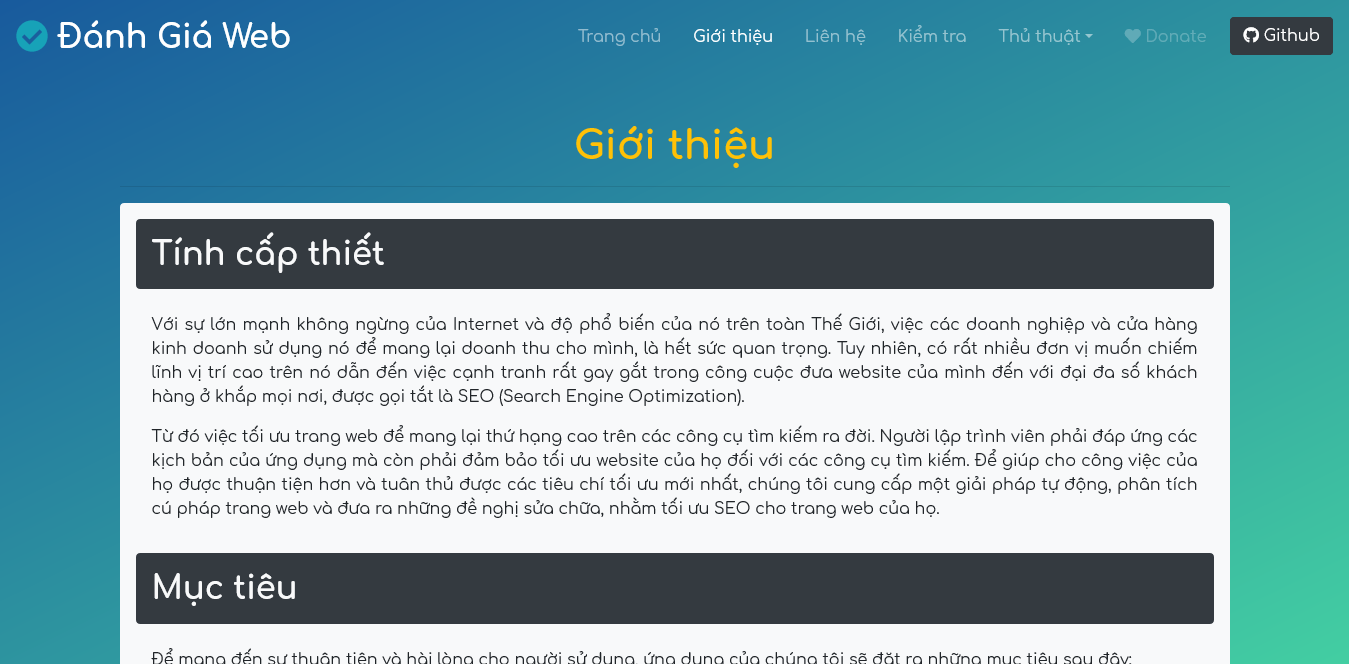
\includegraphics[width=120mm]{images/trang-gioi-thieu.png}
        \caption{Trang giới thiệu của ứng dụng}
    \end{figure}
\end{center}
\begin{center}
    \begin{figure}[!ht]
        \centering
        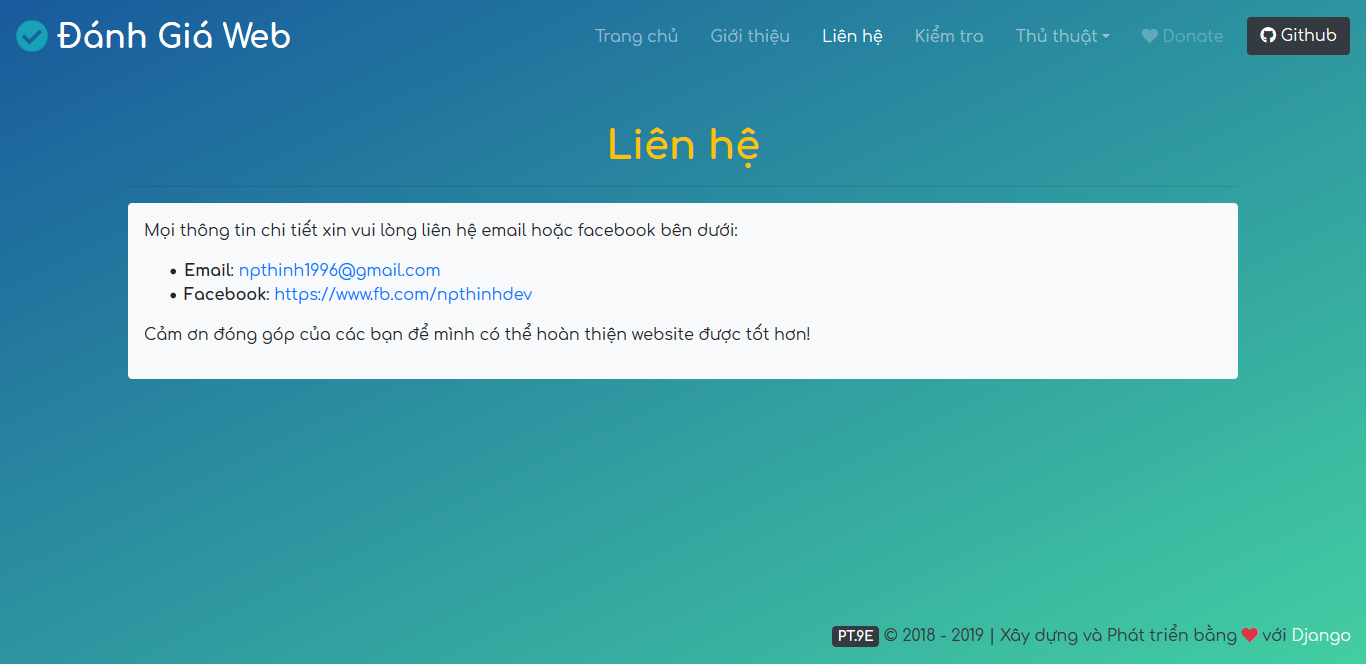
\includegraphics[width=120mm]{images/trang-lien-he.png}
        \caption{Trang liên hệ của ứng dụng}
    \end{figure}
\end{center}
\begin{center}
    \begin{figure}[!ht]
        \centering
        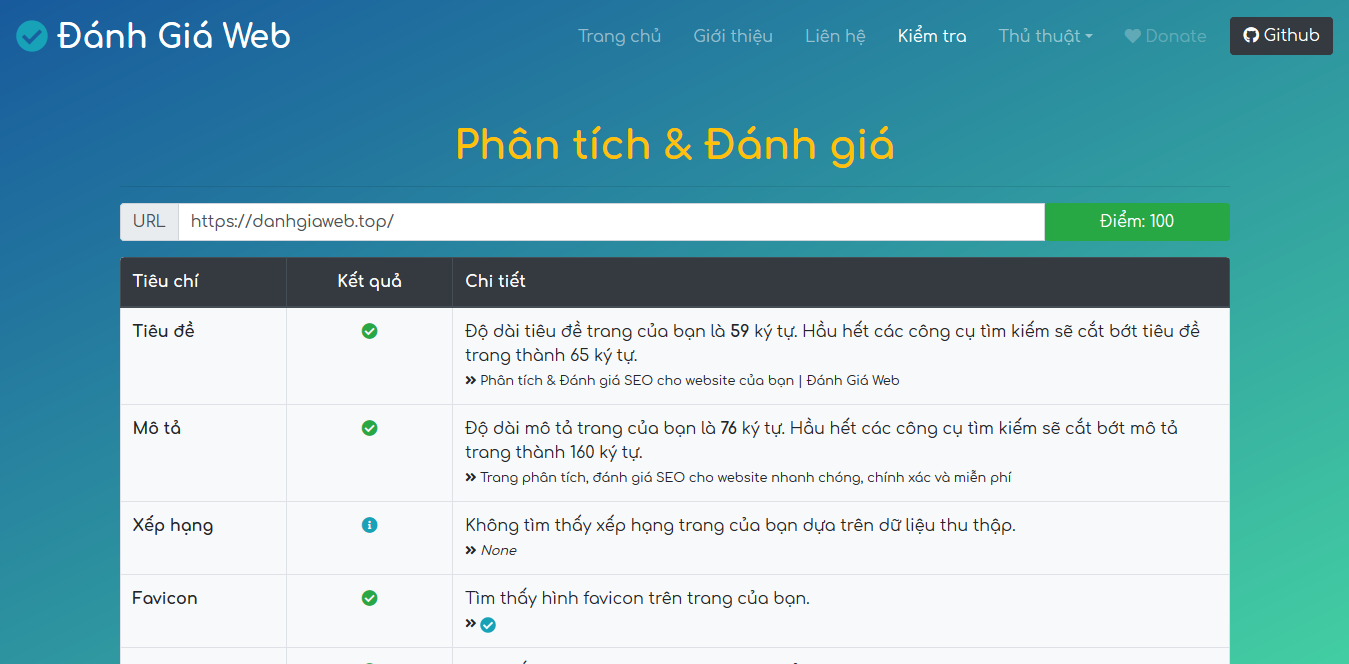
\includegraphics[width=120mm]{images/trang-phan-tich.png}
        \caption{Trang phân tích của ứng dụng}
    \end{figure}
\end{center}
\begin{center}
    \begin{figure}[!ht]
        \centering
        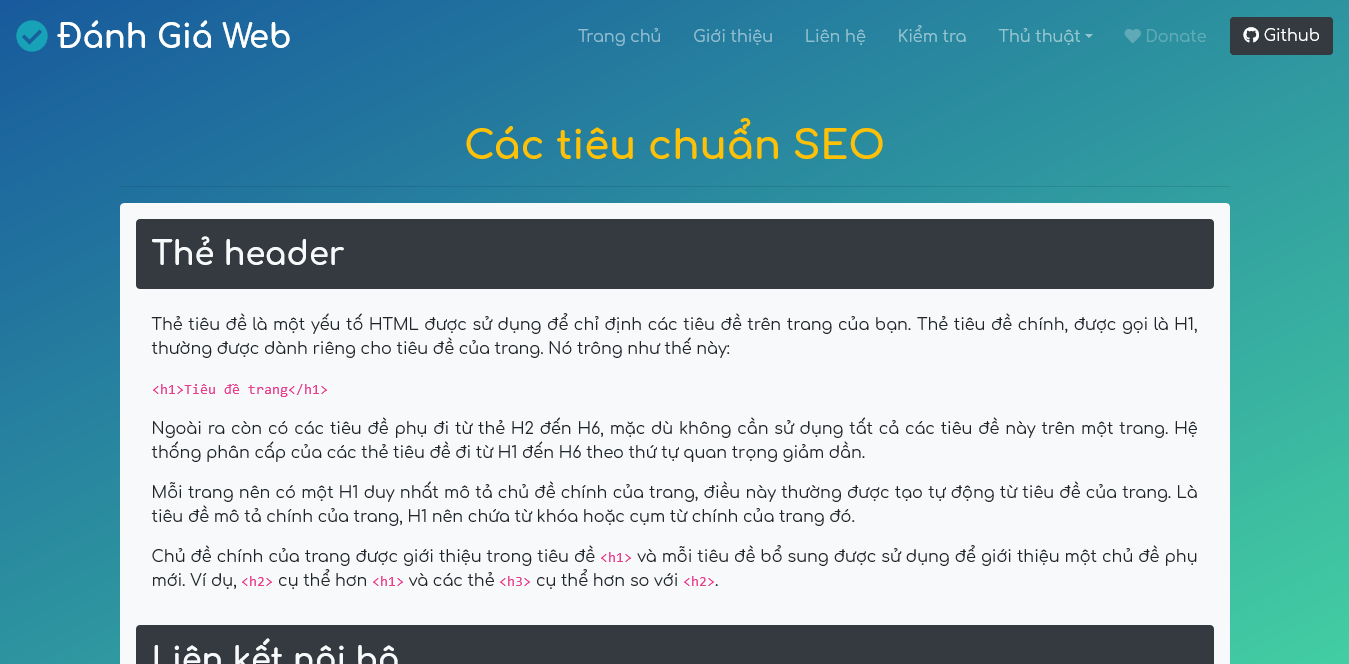
\includegraphics[width=120mm]{images/trang-thu-thuat.png}
        \caption{Trang thủ thuật của ứng dụng}
    \end{figure}
\end{center}
\begin{center}
    \begin{figure}[!ht]
        \centering
        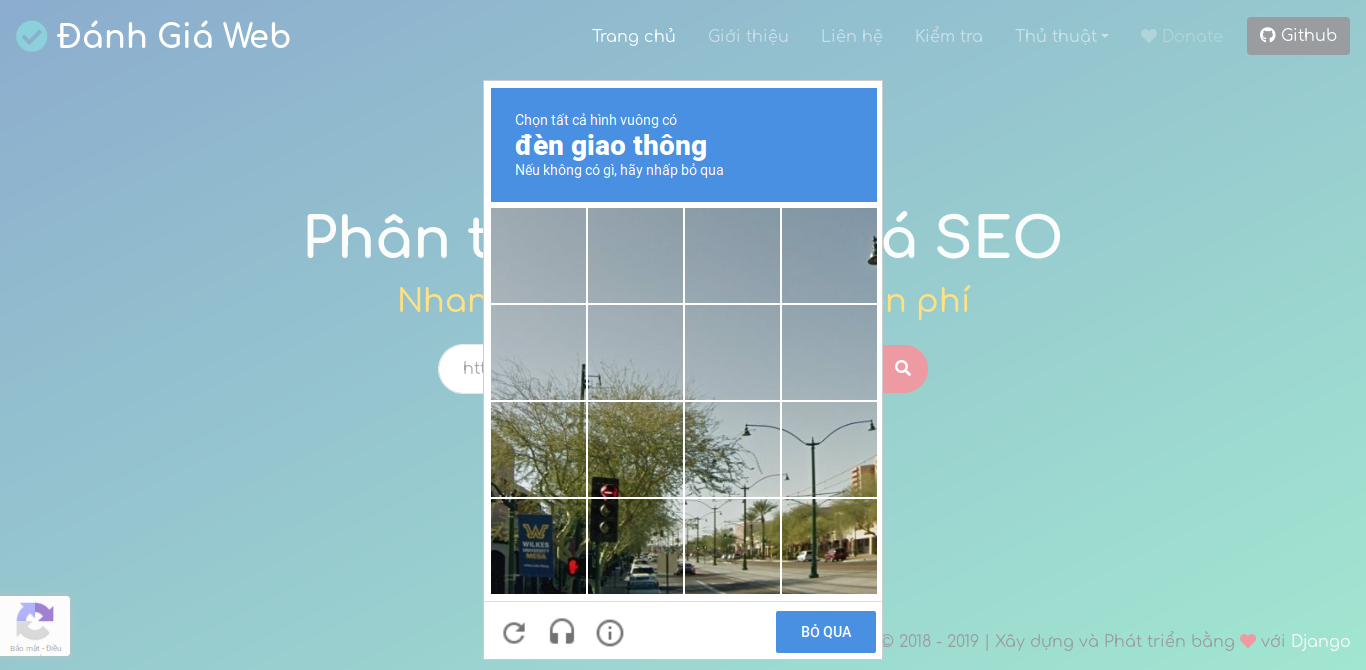
\includegraphics[width=120mm]{images/trang-recaptcha.png}
        \caption{Trang kiểm tra reCaptcha của ứng dụng}
    \end{figure}
\end{center}